\section{Demo}
We build this sequence-based non-projective dependency parser and the part of
the work is licensed under the GNU General Public License.

%\subsection{Experiments}
We evaluate our demo systsem on the WSJ test set under english\footnote{the training set is sections 2-21 of WSJ corpus and test set is sections 00-01} and five non-projective treebanks in different
languages.\footnote{\urlstyle{same}\url{http://ilk.uvt.nl/conll/post_task_data.html}}
\footnote{\urlstyle{same}\url{http://www.nltk.org/nltk_data/}}


\tabref{tab:multilingual test} shows the results of our system(nonproj), MaltParser and MSTParser. Generally, we outperform MaltParser in non-projective treebanks,
which indicates that our framework tolerates free word order better.
Our accuracy is not as good as MSTParser, because of the greedy decoding strategy.
Nevertheless, this strategy gives rise to improvement in
parsing time and flexibility in defining high order features than MSTParser.
\begin{table}[th]
\small
    \centering
    \caption{End-to-end accuracies on 8 languages}
    \begin{tabular}{l|ccc}
        %\toprule
        \whline
        Language & nonproj & MSTParser & MaltParser \\
        %\midrule
        \hline
        basque & 77.45\% & 81.81\% & 74.88\% \\
        dutch & 81.43\% & 85.66\% & 77.28\% \\
        danish & 86.84\% & 89.39\% & 85.65\% \\
        portuguese & 86.93\% & 88.63\% & 85.97\% \\
        slovene & 78.26\% & 80.16\% & 76.09\% \\
        %catalan & 80.22\% & 82.18\% & 79.84\% \\
        %swedish & 87.11\% & 88.12\% & 87.46\% \\
        WSJ & 89.50\% & 90.64\% & 90.23\% \\
        %\bottomrule
        \whline
    \end{tabular}%
    \label{tab:multilingual test}%
\end{table}

Further, we compare the accuracies of the
non-projective arcs in the test data in \tabref{tab:nonproj}.
%The result shows our advantage over non-projectivity.
%We choose the treebanks with more than 100 non-projective arcs in the test data.
The system produces reasonable accuracies and outperforms MaltParser and MSTParser on parsing non-projective arcs.
%Generally, our framework tolerates free word order better.
%\BF{non-proj experiment}
% Table generated by Excel2LaTeX from sheet 'nonproj'

\begin{table}[th]
\tiny
  \centering
  \caption{Accuracy of non-projective arcs in 5 languages}
    \begin{tabular}{c|ccc|ccc|ccc|ccc|ccc}
    %\toprule
    \whline
    \multirow{2}[4]{*}{\textbf{parser}} & \multicolumn{3}{c|}{\textbf{basque}} & \multicolumn{3}{c|}{\textbf{dutch}} & \multicolumn{3}{c|}{\textbf{danish}} & \multicolumn{3}{c|}{\textbf{portuguese}} & \multicolumn{3}{c}{\textbf{slovene}} \\
\cline{2-16}          & \textbf{correct} & \textbf{total} & \textbf{accuracy} & \textbf{correct} & \textbf{total} & \textbf{accuracy} & \textbf{correct} & \textbf{total} & \textbf{accuracy} & \textbf{correct} & \textbf{total} & \textbf{accuracy} & \textbf{correct} & \textbf{total} & \textbf{accuracy} \\
    %\midrule
    \whline
    nonproj  &225 & 569   &  \textcolor[rgb]{ 1,  0,  0}{0.395431} & 339 & 529   & \textcolor[rgb]{ 1,  0,  0}{0.640832} & 79 & 121   & \textcolor[rgb]{ 1,  0,  0}{0.652893} & 104 & 191   & \textcolor[rgb]{ 1,  0,  0}{0.544503} & 101   & 263   & 0.3840304 \\
    %\midrule
    MaltParser  & 200   & 569   & 0.351494 & 300   & 529   & 0.567108 & 58    & 121   & 0.479339 & 103   & 191   & 0.539267 & 98    & 263   & 0.3726236 \\
    %\midrule
       MSTParesr& 204   & 569   & 0.358524 & 204   & 529   & 0.385633 & 63    & 121   & 0.520661 & 90    & 191   & 0.471204 & 109 & 263   & \textcolor[rgb]{ 1,  0,  0}{0.4144487} \\
    %\bottomrule
    \whline
    \end{tabular}%
  \label{tab:nonproj}%
\end{table}%

\cut{
Graph-based method gives a better results for non-projective parsing
than Malt, since it directly scores all arcs between every two nodes.
}

%\subsection{System setup}

Given a CoNLL formatted training data and test data, our demo can parse out the dependency tree.
\figref{fig:workflow} is the snapshot of the demo showing
the parsing result on the multilingual corpus.

\begin{figure*}[th]
\centering
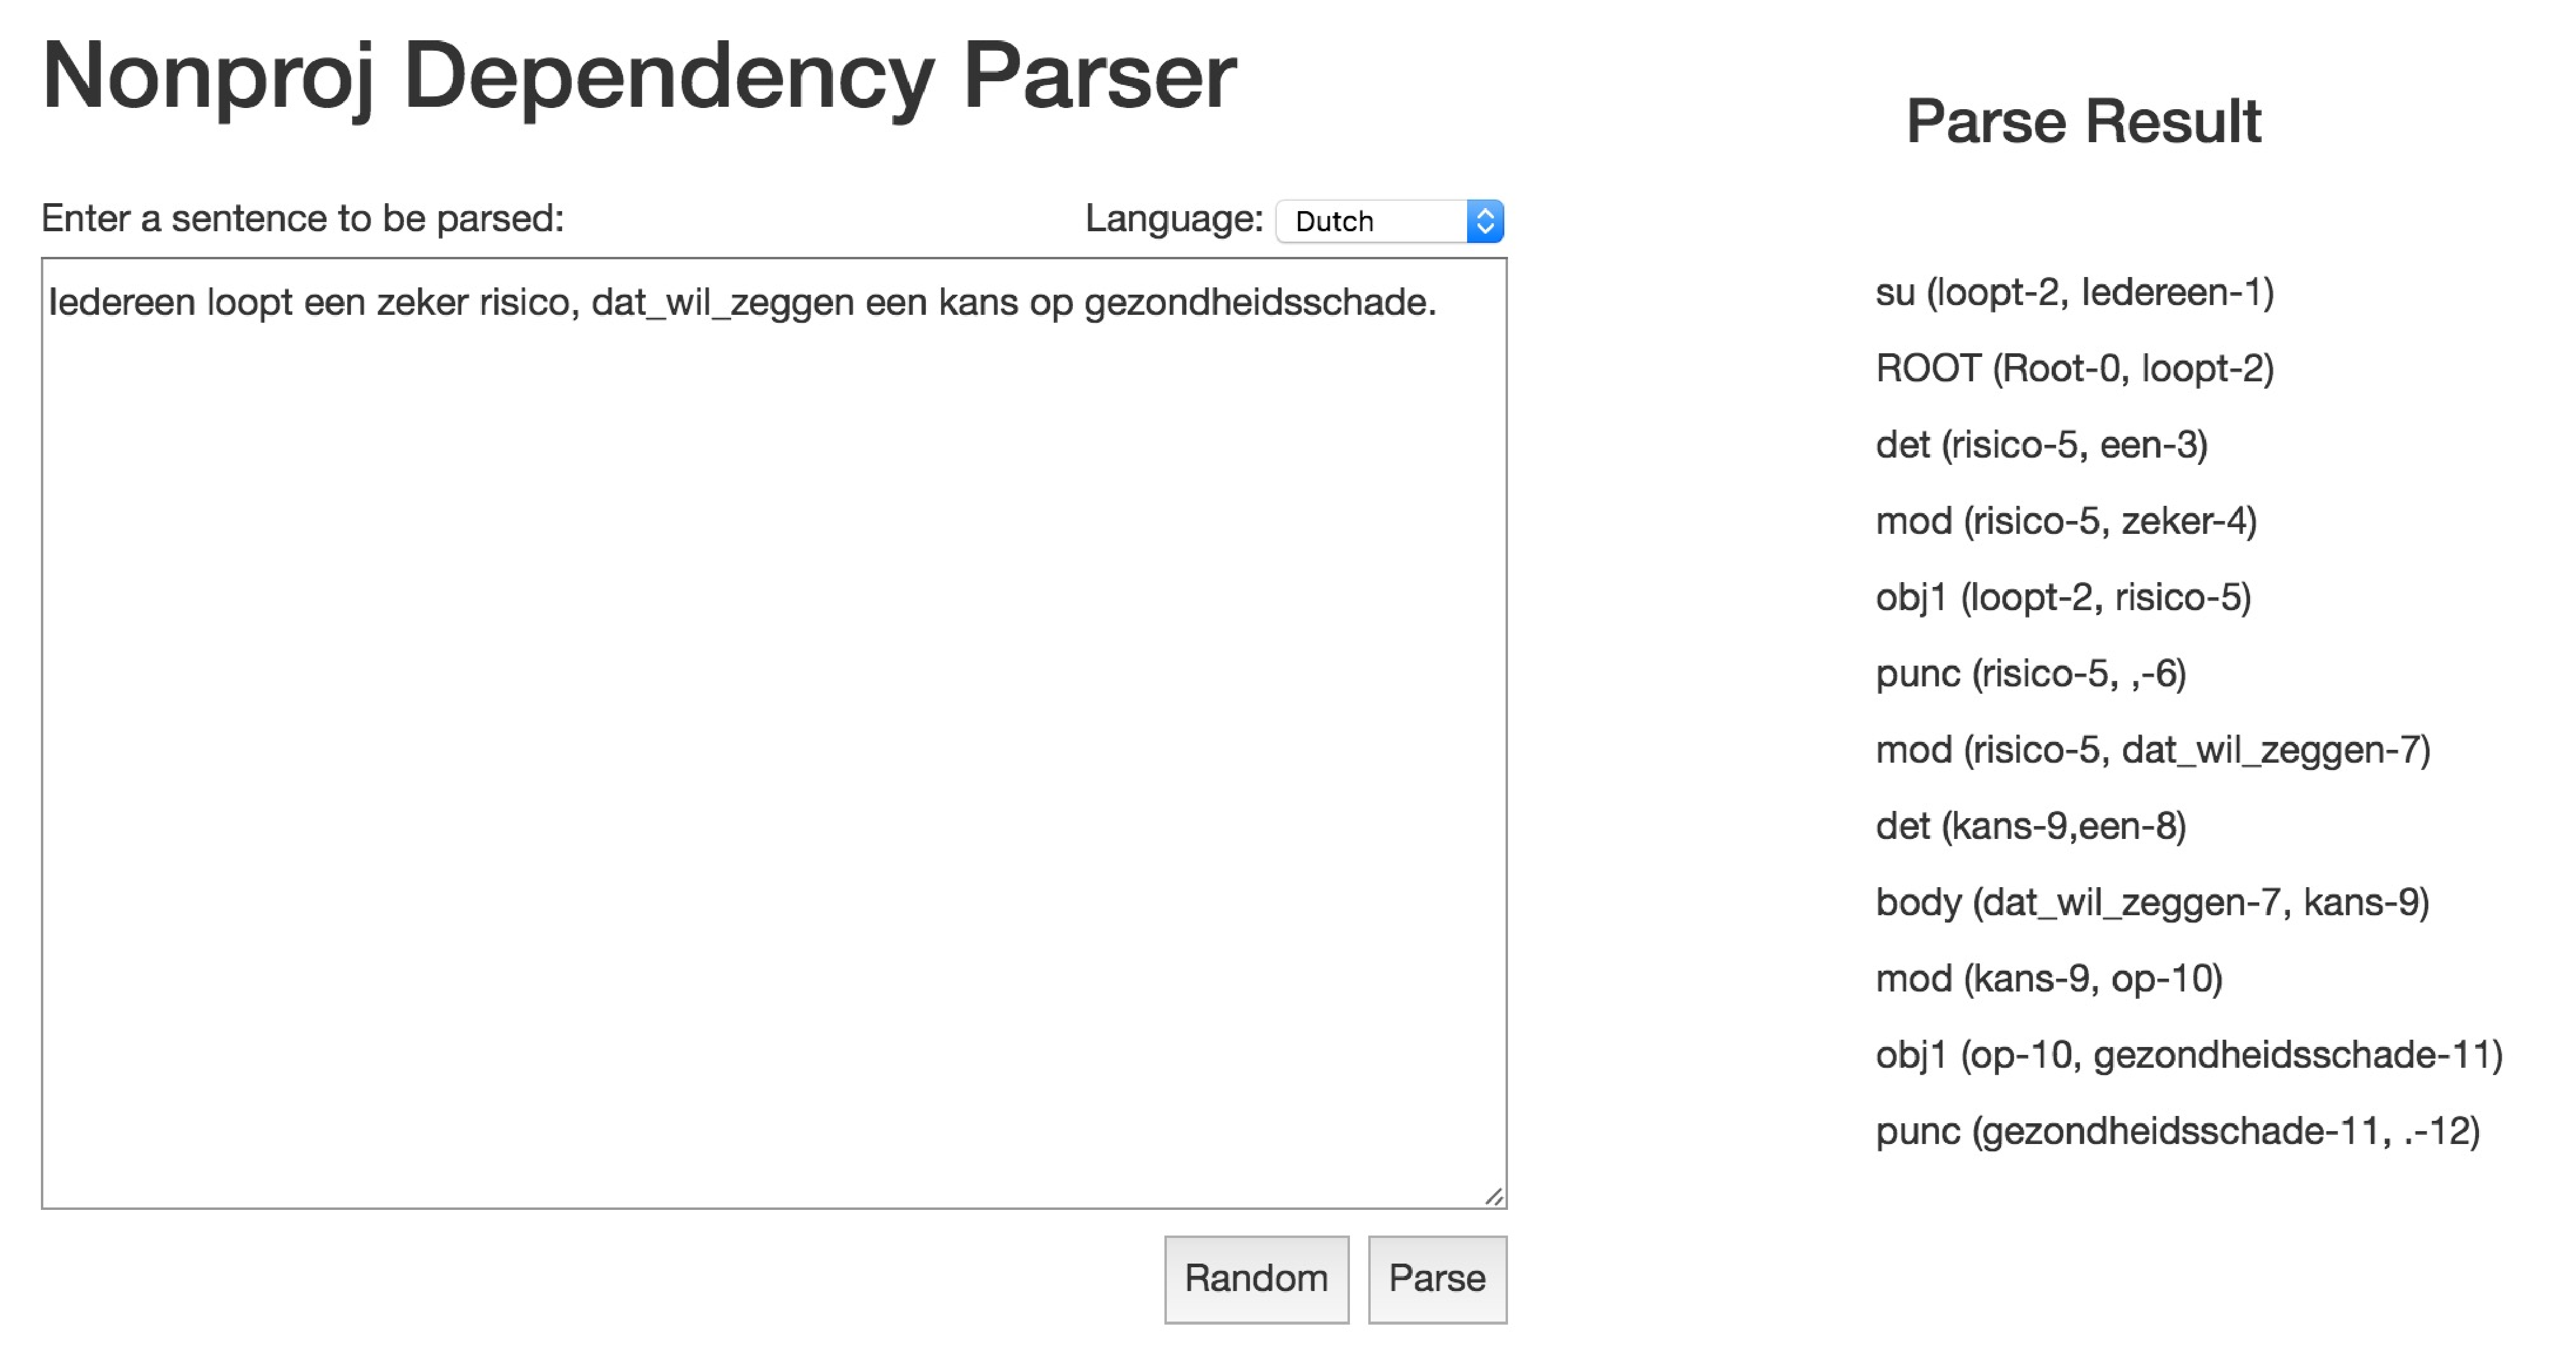
\epsfig{file=nonprojdemo.eps, width=0.9\columnwidth}
\caption{Example Parse of head mapper}
%for the sentence ``\emph{John saw a dog yesterday which was a Yorkshire Terrier}". Red node is the child to be processed in every step; red arc is the final attachment from head to its dependent and dashed arc is left out to avoid circle in the parse tree.}
\label{fig:nonprojdemo}
\end{figure*}
